\section{Implementation}
In upcoming section following expressions will be used:

\begin{tabular}{ll}
$n$ & number of nodes\\
$m$ & number of edges \\
$z$ & number of zones\\
$p$ & number of path computed for one pair of zone
\end{tabular}

Transportation modelling described in previous section was implemented in Python programming language.

\subsection{Static shortest path search}
For determined $C$ we use Dijkstra's algorithm (complexity $O(m +n log(n))$). So final complexity is 
$$z (m + n log(n))$$
For traffic count we used also Dijkstra's algorithm. Final complexity for traffic count is 
$$p z (m + n log(n))$$
For Dijkstra's algorithm we used Python library iGraph. iGraph is written in C programming language so it is fast. For example one Dijkstra running 30 ms ($n = 8000$ $m = 18000$).

\subsection{Data store}
All data for transportation modelling are stored in relation database PostgreSQL with extension PostGIS. In database there are 4 main table:

\begin{tabular}{ll}
roads & road links (edges)\\
nodes & nodes (vertexes)\\
zones & list of zones\\ 
traffic & \\
general\_area\_information & contains interested area geometry\\
od\_pair & Database implementation for $T$ matrix\\
\end{tabular}

\begin{figure}
\centering
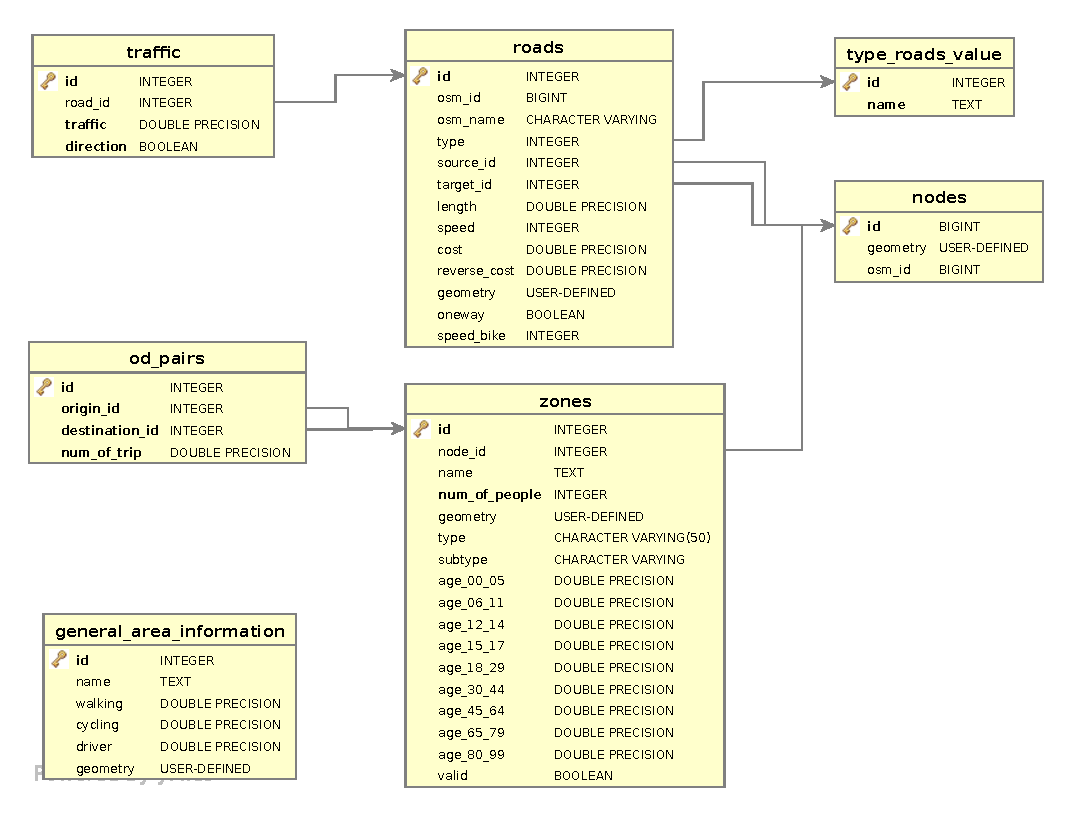
\includegraphics[width=15cm]{img/c01-transp-model/db.eps}
\caption{Database model}
\end{figure}

More details about DB you can find in project documentation on GitHub.
